\chapter{Implementing System Details for Interactive Spatially Augmented Reality}

\fbox{This chapter is still in draft form}

As described in section \ref{tabletop} much of the early work I did in the lab was focused on the virtual heliodon.  The system evolved from a single computer four projector setup to a 3-4 computer setup with 6-8 projectors.  (We have had both 6 and 8 projector setups running on the same infrastructure).
\section{Running the Virtual Heliodon Across Multiple Machines}
The old infrastructure of the system used signals and files to communicate between processes on a single system.  While quick and effective on a single system this strategy did not scale to multiple boxes well.  While file communication across multiple boxes is possible by mounting network drives it is slow and unpredictable in interactive programs.
\subsection{Running radiosity across multiple cores including the BlueGene L}
Because radiosity's bottleneck is computing a form factor matrix, it is naturally very parallelizable.  One attempt to speed up our system was to calculate form factors in parallel and transfer it back to a client for use in lighting.  Part of this was done as a class project with Jon Zolla.  When investigating the existing radiosity solution we discovered that with large meshes (on the order of tens of thousands of polygons), computing form factors could take up to 99\% of the computation time.  Practically, radiosity is very seldom used with meshes of that size for this reason. 

Several optimizations were done too improve the performance of the radiosity solution.
Our original method was simply to divide the number of rows by the number of processors and have each processor compute the rows that it received.  
  The equation for form factors is \fbox{form factor equation here}.  As you can see $F_{ij}$ varies from $F_{ji}$ by only a factor of the areas.  Because of this we decided to only compute the upper right half of the matrix and then calculate the other by multiplying by the factors of the area.  This 
  made our initial division of labor very inefficient as the rows with the most labor were naturally grouped to the same processor while the ones with very little labor were grouped together.  Our solution was to instead divide the number of rows by 2, designate the first half of the matrix to processors like before and have the processor responsible for row i also be responsible for num\_rows-i.  Because we were computing a triangular matrix this worked quite well.  In rooms which are completely open with no occlusion the equation shown above is sufficient, but when rooms have occlusion ray casting is necessary to get accurate renderings.  Ray casting in the context of radiosity is simply shooting a ray from one triangle to another and seeing if any triangles occlude the view.  Unfortunately this computation turns an $O(n^2)$ operation into an $O(n^3)$ operation (go from simply computing $n^2$ form factors to testing n collisions for each).  We reduced this last factor of n by storing 2 resolutions of meshes.  The first mesh was used for radiosity (so we got per triangle accuracy).  The second mesh was used for ray casting occlusion.  Often a mesh of 1/10 the size was available for testing for occlusions and ultimately could speed up the form factor computation by close to that factor (10).  The final improvement we made to the naive algorithm was allowing messages to be received in any order at the end.  It was necessary to have rank 0 assemble the matrix after it was computed.  The naive way to do this is to simply have it first receive row 0 and 1 by 1 go up to row n - 1.  We improved this algorithm by using MPI\_GET\_COUNT to receive variable size messages, therefore allowing the rows to arrive in any order.
 
 We were able to parallelize the radiosity code fairly successfully.  On 256 processors scaling was almost linear.  At 2048, scaling went down to around 64\% of optimal.  While calculating form factors scaled very well, ultimately it was not used in our system because transferring the form factor file back to our system was very slow.   Form factor matrices could reach sizes of 500 MB and transferring these files back to RPI made the system fall quite short of interactive rates.
\subsection{Starting servers and synchronization using MPI}
Because multiple computers became necessary to run the contraption system when we extended it to more than four projectors, a new type of communication architecture was needed.  As radiosity is computationally quite expensive and expensive to transfer form factors we decided on a client server architecture where the server would have much more computational power than the clients.  Multiple clients were needed to run the projectors servers so synchronization need to be achieved by some means.  MPI, Message Passing Interface, provides an effective way to ensure machines running the same code are at the same point: MPI\_Barrier.  Additionally MPI is set up to spawn processes across multiple boxes well.  
MPI also keeps a notion of all existing processes.  An individual processes ID with respect to the other MPI processes is known as rank.  Rank provided us with an easy way to keep track of the processes in the system.  Since each projector has a different perspective into the scene we had to have a separate calibrated camera file for each one.  This calibrated camera file also was fed to the remesher program (made by Barbara Cutler) which outputted blending weights (the part of the scene each projector should project).  Blending weights, camera calibration files and individual processes were all tracked by this idea of rank.
For these reason MPI was used for synchronization across clients as well as starting the client processes.  
\subsection{Communicating via sockets}
Because we wanted our system to capable of projecting applications besides daylighting it was important that the communication between the server and the clients was not limited to a single communication pattern.  I developed a Socket Communicator Class to address this.  The socket communicator class reads things sent via socket to the remote renderers.  It is designed to communicate in two ways: to read commands and to read larger messages such as images.  Common commands include RENDER, UPDATE\_TEXTURE, and FLIP.  Calls such as UPDATE\_TEXTURE would be followed by a compressed (or uncompressed) images.  By having command such as these available, applications like ARmy were able to be used in our system.
Using TCP sockets added an element of complexity to starting our program.  When opening a TCP socket, one process has to be listening for a socket while another attempts to connect to it.  We decided to have the remote renderers first create the socket and wait for an attempted connection.  Sockets were used in the 56000-57000 port window because they are seldom used by the system.  The script starting the system waits 10 seconds after telling the remote renderers to open sockets (as MPI must initialize as well).  The render controller then connects to the remote renderers.

Unfortunately sockets do not allow unlimited information to be sent to them without the information being read from the other side.  This was a point of difficulty with our program as often we want to send textures from the render controller and because it is currently 6 remote renderers to 1 render controller it is not ideal to be waiting for each remote renderer to process information before sending it to the next one.  Sending large images also presented a problem.  Images larger than 512x512 often caused the sockets to stop responding.  Because bandwidth also ended up being a bottleneck, we chose to limit ourselves to 512x512 resolutions for the time being.  We also had the option of tiling 512 by 512 textures across a surface.  In order to make sure that messages being sent do not get too far ahead of those being received, we have rank 0 send an acknowledgment message back to the render controller once for each rendering of a scene.  Depending on the number of textures sent, the relative performance of the computers, the speed of the network, and the number of machines in the system, the frequency of acknowledgment messages will have to be adjusted to ensure the sockets do not become saturated.
\section{Other System details}
I have also performed many smaller tasks as part of keeping the system running well.  The following, while not large research contributions have enabled the system to keep running.
\paragraph{Camera Class}
As the system evolved, we have used different cameras as part of it including both firewire and gigabit ethernet cameras.  Unfortunately, these cameras all have different interfaces.  To attempt to make this an easier thing to adapt an abstract class was developed that could then be implemented for various cameras.  This class included things like initialize camera, get next frame, and get latest frame.  
\paragraph{Bash Scripts}
Because the system has so many programs interacting, we used scripts to bash scripts to tie them together.  Bash scripts allowed us to easily sort debug output based on input parameters.  It also was very helpful in ensuring programs were initiated in the right order.  (Remote renderers need to be initiated before the render controller as described earlier).  For the user studies scripts made the job of administering the study manageable.  Images from the overhead camera, debugging images, renderings, as well as parameters requested by users were all recorded in corresponding folders using our collection of scripts.
\paragraph{Compressed Textures}
In an attempt to reduce bandwidth usage on our network we tried compressing the textures before sending them to the remote renderers.  We chose to use zlib to do the compression.  To do the decompression we just needed to send a header with the height, width and compressed texture size.

 \begin{figure*}[t]
    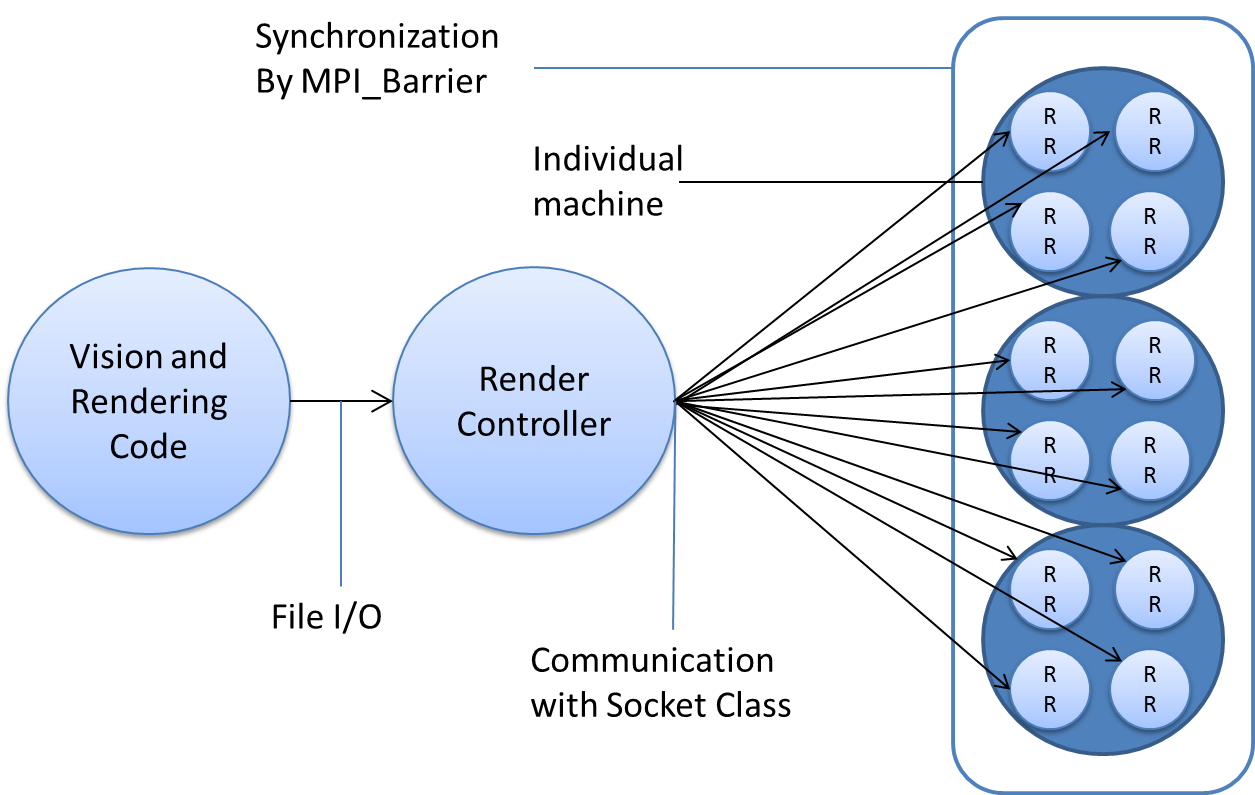
\includegraphics[width=120mm]{images/MPI_socket_diagram.png}%
%\vspace{-0.25in}\\
  \caption[Communication diagram of the Virtual Heliodon System]{ 
%
Communication between the render controller and remote renderers.  The RR's represent the remote renderers.  
Two types of communication are done in this portion of the system: MPI calls and socket communication}
\vspace{-0.15in}
\label{FIGURE:block_diagram}
\end{figure*}
%I have been responsible for much of the system maintenance and development since I joined this project.  When we decided to extend the system to ten projectors for the third visit to EMPAC, the system had to span five computers.  The three computers driving projectors had to be synchronized.  In order to do this, I adjusted some existing rendering code such that it was run in parallel across multiple machines.  Formerly, we were limited to the number of projectors that could be controlled by one machine or having our control be limited to sending signals inside of bash scripts.  



\begin{figure*}[t]
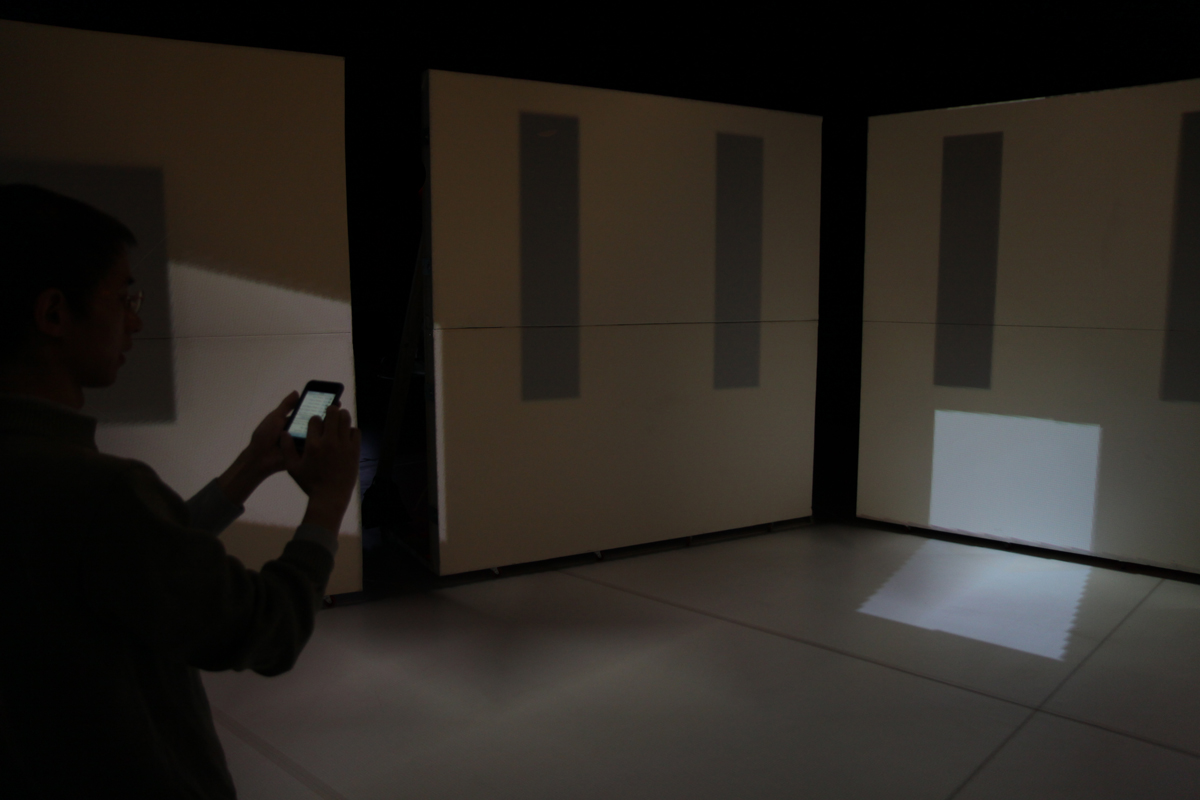
\includegraphics[width=0.5\textwidth]{images/IMG_2092_crop.jpg}
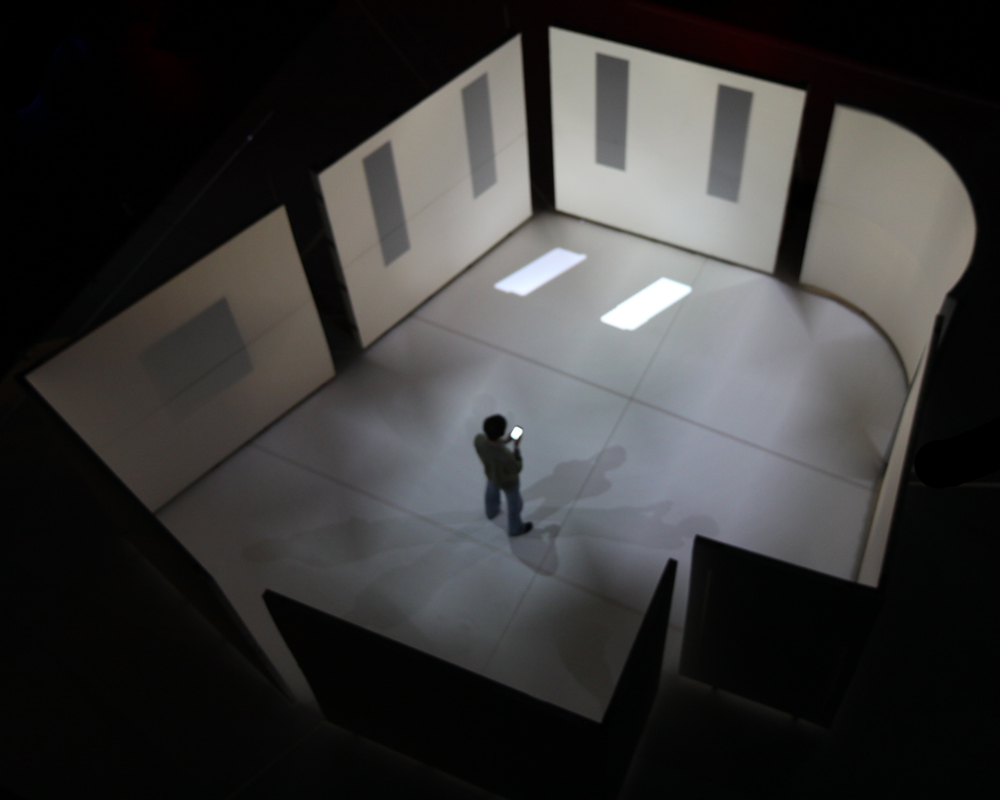
\includegraphics[width=0.5\textwidth]{images/IMG_2119_crop.jpg}

\caption{Example daylighting images from the full scale virtual heliodon}

\end{figure*}
\section{Summary}
While not involved in the original design of the tabletop heliodon, I was responsible for much of the implementation details involved in extending the system to multiple machines using more projectors.  Much of this was closely tied to the communication required between the system including sending commands and textures and synchronization.

